%focus on sub-goal
\chapter{Design and Implementation}\label{chapter:prototype_implementation}

Implementing an \gls{ea} requires a number of considerations. A robust fitness assignment method needs to be determined. A mechanism for uniform diversity preservation must be conceptualized, and a well-thought-out solution to address constraints in the problem definition must be designed. There are successful \glspl{ea} that can be used for this; these algorithms have been well researched, and their domain applicability is well defined.

\Gls{nsga}-II \parencite{Jain2013AnOptimization} is an \gls{ea} that uses an elitist non-dominated sorting mechanism to approximate the Pareto front. It is an improved version of an initial \gls{nsga} algorithm developed by Srinivas et al. \parencite{Srinivas1994MuiltiobjectiveAlgorithms} in 1996. 
\Gls{nsga}-II uses crowding function for diversity preservation and ranking of the Pareto fronts. However, it is better suited for two-objective problems and does not perform well on multi-objective problems. \Gls{nsga}-III \parencite{Mkaouer2015Many-objectiveNSGA-III} was introduced to address the inability of \gls{nsga}-II to solve multi-objective problems (i.e., three or more objectives).

Other successful \glspl{ea} applicable to our problem can be found in practice. In the following sections, we implement the \gls{nsga} algorithm and its heuristic adaptations to suit our problem definition.

\section{Non-Dominated Sorting Genetic Algorithms}
Designing domination-based \gls{emo} algorithms for multi-objective problems requires additional considerations. For instance, an increase in the number of objectives may cause an increase in the non-dominated population derived from the randomly generated population. Since domination-based \gls{emo} prioritizes non-dominated solutions, the solution space becomes rather large. Therefore, the search process becomes slow, and the algorithm becomes inefficient. With increased solution space also arises an increase in the number of neighbors. Evaluation of diversity measures (i.e., crowding distance) becomes computationally expensive. \Gls{nsga}-III was designed to address these problems.

As defined in \ref{sec:problem_definition}, our problem can be mapped to many objective optimization problems. Each objective function is a function of a \gls{poi} and its characteristics. A chosen algorithm needs to efficiently compare more than three objectives, and this informs the decision to implement and adapt the \gls{nsga}-III to our problem domain. Next, we explore the aspects that comprise the \gls{nsga}-III and constitute our algorithm.


\subsection*{The \Gls{nsga}-III Algorithm}
The \gls{nsga}-III algorithm was developed to address the inefficiency of \gls{nsga}-II in handling multi-objective problems. In its most basic form, \gls{nsga}-III can be seen as the \gls{nsga}-II algorithm with minor changes; that is, most algorithmic steps in \gls{nsga}-III are from the \gls{nsga}-II algorithm. Figure \ref{fig:nsgaII} and \ref{fig:nsgaIII} depict an overview of the major algorithmic steps in \gls{nsga}-II and \gls{nsga}-III, respectively. From these figures can be observed the similarity between the two algorithms. However, a major difference between them is in the last step of next-population generation. Unlike \gls{nsga}-II, which sorts individuals by crowding distance to decide what part of a Pareto front to reject or accept, \gls{nsga}-III uses a sorting technique based on a reference point. Sorting by crowding distance is explained in Section \ref{sec:diversitypreservation}. The reference-point-based sorting technique and other intrinsic details of the \gls{nsga}-III are explained below.

\begin{figure}
    \centering
    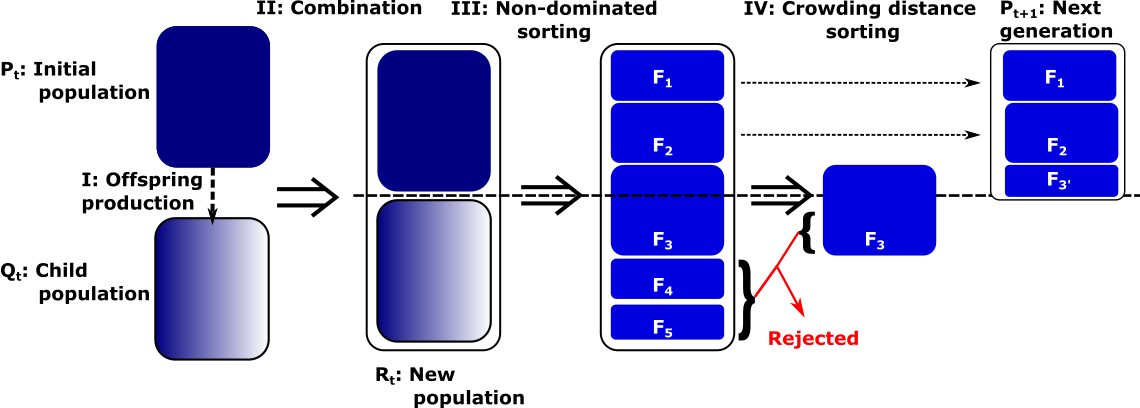
\includegraphics[width=9cm]{NSGA-II}
    \caption{\gls{nsga}-II overview}
    \label{fig:nsgaII}
\end{figure}

\begin{figure}
    \centering
    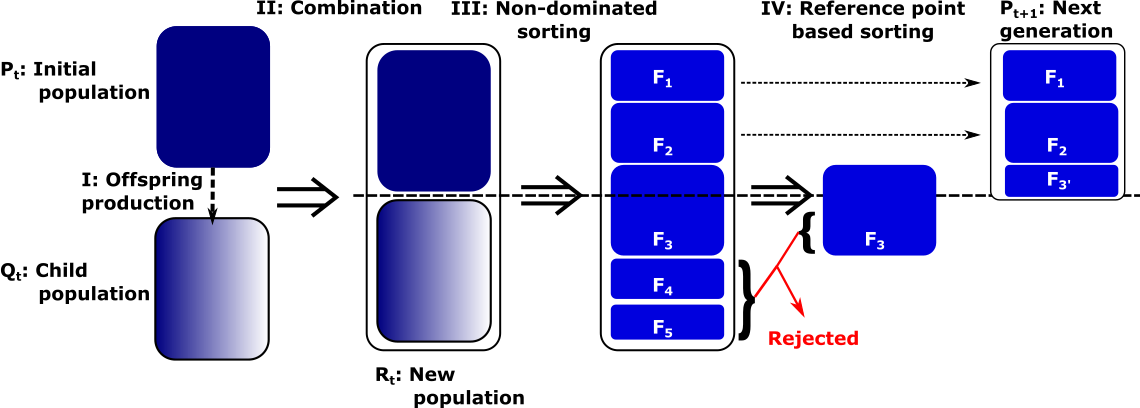
\includegraphics[width=9cm]{NSGA-III}
    \caption{\gls{nsga}-III overview}
    \label{fig:nsgaIII}
\end{figure}

\subsubsection{Initial Population}
Let us consider $P_t$ as a parent population of the $t^{th}$ generation of the algorithm (i.e., iteration $t$). $P_t$ with $N$ chromosomes is either a population taken from previous generation  $t-1$ or an initial population taken from a defined heuristic.\\ 
The heuristic used for initial population generation at the start of the algorithm is particularly important for our problem. Simply sampling randomly from the problem space would be logically inefficient. The number of objective problems in practice is typically capped at 15–20. \Gls{nsga}-III was evaluated on 20-objective DTLZ1-DTLZ2. Considering that the objective function in our problem domain comprises a single \gls{poi} and its characteristics, an intelligent pre-selection process must be defined to reduce the problem space.

\subsubsection{Constraint Handling}\label{sec:sub_conshandling}
Figure \ref{fig:unconstrainedsearchspace} illustrates a typical solution search space for an unconstrained problem. For unconstrained problems, all members of the population are regarded as feasible; however, some individuals can become infeasible (i.e., members in the gray shaded area; Figure \ref{fig:constrainedserachspace}), some individuals become infeasible (i.e., members in gray shaded area). Additional techniques are required for handling constraints in \gls{nsga}-III. Two papers address problems with \gls{nsga}-III both with \parencite{Deb2013AnConstraints} and without \parencite{Jain2013AnApproach} constraints. 

\begin{figure}[h!]
\centering
\subfloat[Unconstrained solution search space]{
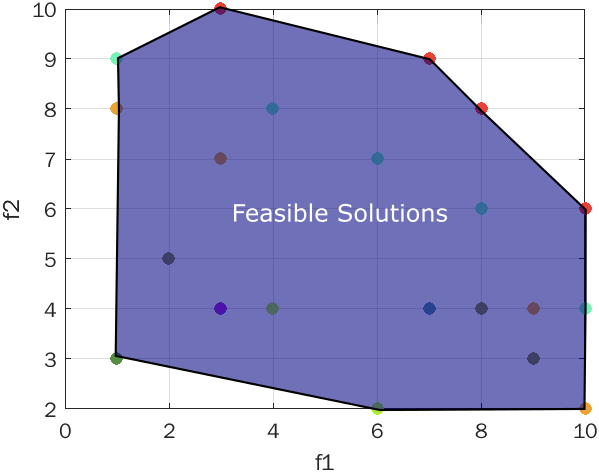
\includegraphics[width=.4\textwidth]{UnconstrainedSolutionSpace}
\label{fig:unconstrainedsearchspace}}\qquad
\subfloat[Constrained solution search space]{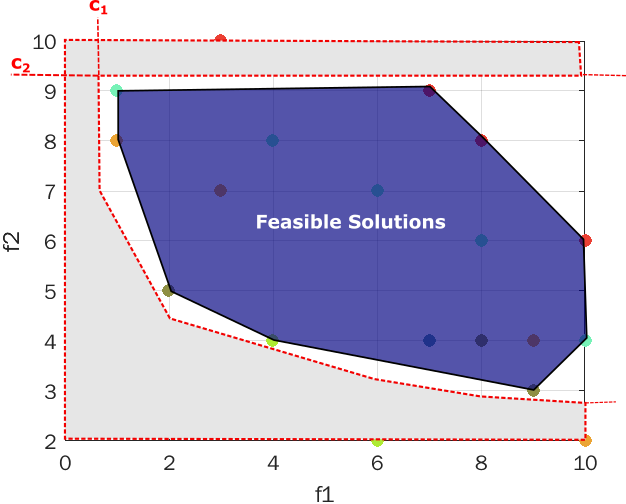
\includegraphics[width=.4\textwidth]{ConstrainedSearchSpace}
\label{fig:constrainedserachspace}}
\caption{Solution Search Space}
\label{fig:constrainedvsunconstrained}
\end{figure}

Consider an individual $x$ in the solution space with the following constraints:

\begin{align}
    \tag{constraint 1 }g_j(x) \leq b_j \label{eq:4a}\\
    \tag{constraint 2}h_k(x) = 0 \label{eq:4b}
\end{align}

The authors of \parencite{Jain2013AnApproach} suggest calculating a constraint valuation value $CV(x)$ to measure the degree to which $x$ violates the constraints using the following formula:

\begin{align}
    \tag{1}CV(x) = \sum_{j=1}^J \langle g'_j(x)\rangle + \sum_{k=1}^K \lvert h'_k(x)\rvert \label{eq:4c}
\end{align}

where $g'_j(x)$ is the normalized constraint function for Constraint \ref{eq:4a}, such that $g'_j(x) = g_j(x) / b_j  - 1 \leq 0$ and $h'_k(x)$ is the normalized constraint function for Constraint \ref{eq:4b}. The angle bracket operator $\langle \alpha \rangle$ returns the negative of $\alpha$, if $\alpha < 0$ and returns zero, otherwise. Assuming that Constraint \ref{eq:4a} is a greater or equal constraint (i.e., $g_j(x) \geq b_j$), then $\langle \alpha \rangle$ returns the negative of $\alpha$, if $\alpha > 0$ and returns zero, otherwise.

The notion of feasibility together with the constraint violation measure $CV(x)$, are combined to derive a constraint domination principle. Consider two individuals $x_1$ and $x_2$ in the solution space. An individual $x_1$ is said to constraint dominate $x_2$ if any of the following conditions holds:
\begin{enumerate}
    \item $x_1$ is feasible and $x_2$ is infeasible;
    \item Both $x_1$ and $x_2$ are infeasible and $x_1$ has a lower \gls{cv} value; or
    \item Both $x_1$ and $x_2$ are feasible and $x_1$ dominates $x_2$ ($x_1 \succ x_2$).
\end{enumerate}




\subsubsection{Offspring Production}
Three major aspects in generating the child population $Q_t$ are defined as follows:

\begin{enumerate}
    \item \textbf{Tournament Selection}: To select two individuals that will be eligible to produce offspring for the next generation, a tournament selection procedure is carried out. Two individuals are selected at random from $P_t$, and a binary selection of the better solution is applied, as shown in Algorithm  \ref{alg:tournament_selection}. Individuals $p_1$ and$p_2$ are compared to select the one that does not violate the constraints. If both individuals violate the constraints, the constraint violation values for the two individuals are computed. Then, the algorithm selects the individual with the lesser constraint violation value. Two parents for reproduction (crossover and mutation) are selected using this tournament procedure.
    \item \textbf{Cross over}: A crossover operator is used to generate offspring according to a crossover rate $p_c$. The crossover rate represents the proportion of parents on which a crossover operator will act. A uniform crossover ensures that each offspring will inherit some characteristics of both parents. Either the 1-point crossover or the n-point crossover is commonly used for binary representations. When using the 1-point crossover, a crossover site $k$ is randomly selected. is randomly selected. Then, two offspring are created by exchanging the segments of the parents \parencite{Talbi2009Metaheuristics:Implementation}. Consequently, n-point crossover implies $n$ crossover sites.
    %The most commonly used rates are in the interval [0.45, 0.95]. Adaptive techniques for the crossover rate may also be useful
    \item \textbf{Mutation}: Mutation operators act on a single individual. An element of the representation is mutated (changed) according to some probability $p_m$. \parencite{Talbi2009Metaheuristics:Implementation} recommends small values for $p_m$ ($p_m \in [0.001, 0.01]$). A flip operator is commonly used when using binary representations of individuals. %Some strategies initialize the mutation probability to 1/k where k is the number of decision variables, that is, in average only one variable is mutated.
    
\end{enumerate}
During reproduction, duplicate offspring are checked and eliminated. A child population $Q_t$ of size $N$ is generated by repeating tournament selection and reproduction. $R_t$ is generated by combining $P_t$ and $Q_t$ (i.e., $R_t = P_t \cup Q_t$). \Gls{nsga}-III and \gls{nsga}-II use an elitist preservation technique (III and IV in figure \ref{fig:nsgaIII}) to preserve elite members of the new population.

\begin{algorithm}[h!]
  \caption{Tournament selection procedure in  constrained \gls{nsga}-III}\label{alg:tournament_selection}
  \SetKwInOut{Input}{Input}
  \SetKwInOut{Output}{Output}
  \Input{$p_1$, $p_2$}
  \Output{$p'$}
    \uIf{feasible($p_1$) and not feasible($p_2$)}
    {
        $p' = p_1$
    }
    \ElseIf{not feasible($p_1$) and feasible($p_2$)}
    {
        $p' = p_2$
    }
    \ElseIf{not feasible($p_1$) and not feasible($p_2$)}
    {
        \If{CV($p_1$)  $>$ CV($p_2$)}
        {
            $p' = p_2$
        }
        \ElseIf{CV($p_1$)  $<$ CV($p_2$)}
        {
            $p' = p_1$
        }
        \Else{
            $p' = random(p_1, p_2)$
        }
    }
    \ElseIf{feasible($p_1$) and feasbile($p_2$)}
    {
        $p' = random(p_1, p_2)$
    }
    
  \end{algorithm}

\subsubsection{Non-Dominated Sorting} \label{sec:sub:nondominatedsorting}
Non-dominated sorting ranks members of the population $R_t$ into different non-dominated levels ($F_1$, $F_2$, and so on). In optimization problems without constraints, the sorting is performed using individuals fitness values, while in optimization problems, individuals are ranked according to their constraint domination count. We introduce a new symbol $\succ_+$ for constraint domination. For example, let $A$, $B$, and $C$ be selected members of the population  such that $A \succ_+ B \succ_+ C$ (i.e., individual $A$ constraint dominates individual $B$ and $C$, individual $B$ constraint dominates $C$). Figure \ref{fig:paretolevels} depicts $A$, $B$, and $C$ on a graph. $A$ has the highest domination count and hence belongs to domination level $F_1$. $B$ and $C$ belong to level $F_2$. 

\begin{figure}
\centering
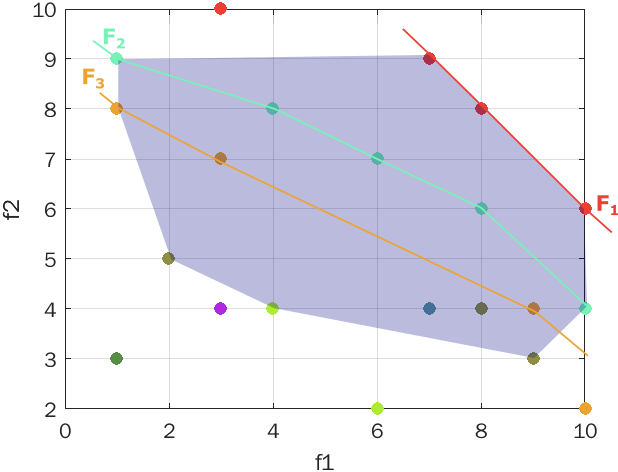
\includegraphics[width=.5\textwidth]{NonDominatedFronts}
\caption{Ranking of Pareto Frontier according to Constrained Domination}\label{fig:paretolevels}
\end{figure}

Thereafter, the number of feasible solutions $N_f$ in $R_t$ are counted. If $N_f \leq N$, all the feasible solutions are added to $S_t$ to start the next generation $P_{t+1}$. The remaining $K = N - \lvert P_{t+1} \rvert$ population slots are filled with top-level infeasible solutions, that is solutions having smaller \gls{cv} values.\\
If $N_f > N$, the algorithm follows the unconstrained selection procedure described in \parencite{Deb2013AnConstraints}. Each level is selected one at a time until a size $N$ is reached or $N$ is exceeded for the first time. Assuming the $l^{th}$ level is the level that causes the size of $S_t$ to exceed $N$, then solutions in level $l$ are only partially accepted into $S_t$. 
%niche-preservation operator that computes the crowding distance for every last level member as the summation of objective-wise normalized distance between two neighboring solutions. 

\subsubsection{Reference Point-Based Sorting}
\Gls{nsga}-III uses a pre-defined set of reference points to ensure diversity in solutions. The reference points can either be preferential points supplied by the user or pre-defined in a structured manner \parencite{Deb2013AnConstraints}. \\ 
In the case of structured reference points, \gls{nsga}-III uses a systematic approach that creates points on a normalized hyperplane. Points are placed on the hyperplane with the same orienteering in all axes. The total number of reference points ($H$) is given by the following:
\begin{align*}
    H &= \begin{pmatrix}
    M + p - 1 \\
    p
    \end{pmatrix}
\end{align*}
where $M$ is the number of objective functions, and $p$ is the number of divisions to consider along each objective. For example, using three objectives ($M = 3$) and four divisions ($p = 4$), the reference points are placed on a triangle with its apex at $(1,0,0), (0,1,0),$ and $(0,0,1)$. $H = \big(\begin{smallmatrix}
  6\\
  4
\end{smallmatrix}\big)$, so 15 reference points are created. The obtained reference points are widely distributed on the entire normalized hyperplane, and the solutions are widely distributed on or near the Pareto-optimal front. Population members associated with the created reference points are emphasized. The population size is recommended to be the smallest multiple of four that is greater than $H$. In the case of user-supplied reference points, the user can mark $H$ points on the normalized hyperplane.

After determining the reference points on a hyperplane, the algorithm adaptively normalizes the population members. First, the ideal point\footnote{The algorithm presented in the paper focused on minimization problems, thus the ideal point was differently defined. Since, we are faced with a maximization problem, our ideal point is defined differently.} of the population $S_t$ is determined by identifying the maximum value ($z_i^{max}$) for each objective function $i = 1, 2,...., M$ in $\cup_{\tau=0}^{t} S_\tau$ and by constructing the ideal point $\Tilde{z} = (z_1^{max}, z_2^{max},..., z_M^{max})$. Using $f'_i(x) = z_i^{max} - f_i(x)$, each objective value of $S_t$ is translated. Thereafter, the extreme point ($z_i^{ext}$) in each objective axis is identified. Given  a weight vector $d_i$, that is close to the $i^{th}$ objective axis, an achievement scalarizing function (ASF) is given by the following:
\begin{align*}
    ASF(x, d_i) = max_{k=1}^M \frac{f'_i(x)}{d_i}, \qquad for\ i = 1, 2,...,M. 
\end{align*}
$z_i^{ext}$ is identified by finding a solution ($x \in S_t$) that results in the minimum corresponding ASF. These $M$ extreme vectors are then used to represent an $M$-dimensional hyperplane. The intercept $a_i$ of the $i^{th}$ objective axis and the linear axis can then be calculated by $a_i = z_i^{max} - z_i^{ext}$. These maximum and extreme values are updated at every generation using the current population. Putting this all together, the objective function can be normalized using the following:

\begin{align}
    f_i^n(x) &=  \frac{z_i^{max} - f_i(x)}{z_i^{max} - z_i^{ext}}, \qquad for\ i = 1, 2,...,M. \label{eq:41a}  
\end{align}

After normalizing the objective functions, each population member is associated with a reference point. A reference line for each reference point on the hyperplane is defined by joining the reference point with the ideal point. Then, a perpendicular distance between each population member and each reference line is calculated. The reference point that has the closest reference line to a population individual in the normalized objective space is considered to be associated with the population individual.

A niche-preserving procedure to generate the remaining $K = N - \lvert P_{t+1} \rvert $ population slots is performed. population slots is performed. A reference point may have one or more population members associated with it, or there might not be any associated reference point. Initially, the population members from $P_{t+1} = S_t \setminus F_l$ that are associated with the $j^{th}$ reference point are counted as $\rho_j$ (niche count). Then, the reference point set $J_{min} = {j:argmin_j \ \rho_j}$ having minimum $\rho_j$ is identified. In case of multiple such reference points, a random $\Tilde{j} \in J_{min}$ is selected from $J_{min}$. 
If there is no associated $P_{t+1 }$ member to the reference point $\Tilde{j}$ ($\rho_{\Tilde{j}} = 0$), then either of the following scenario is possible: 
\begin{enumerate}
    \item There exists one or members in front $F_l$ that are associated with the reference point $\Tilde{j}$, or
    \item The front $F_l$ does not have any member associated with the reference point $\Tilde{j}$.
\end{enumerate}
In case 1, the first case, the reference point with the shortest perpendicular distance from the reference line is added to $P_{t+1}$; then, the count $\rho_{\Tilde{j}}$ for the reference point $\Tilde{j}$ is incremented by 1. In case 2, the reference point is excluded from further consideration for the current generation.\\
In the event that $\rho_{\Tilde{j}} \geq 1$, a randomly chosen member (if one exists) from the front  $F_l$ associated with the reference point $\Tilde{j}$ is added to $P_{t+1}$. The count $\rho_{\Tilde{j}}$ for the reference point $\Tilde{j}$ is incremented by 1. The procedure is repeated $K$ times until all vacant slots in $\rho_{\Tilde{j}}$ are filled.



\section{Implementation and Algorithmic Approaches}\label{sec:impl}
In this section, details of the implementation and several approaches to solving the many objective \glspl{op} discussed in Section \ref{sec:problem_definition} are presented. Our approach consists of an optimization process that comprises varying initialization steps and constraint-handling techniques. Algorithm \ref{alg:opt_framework} outlines the general structure of the approach, which addresses both initialization and the constraint-handling technique. It is important to note a fundamental difference between the non-dominated sorting explained in Section \ref{sec:sub:nondominatedsorting} and outlined in Algorithm \ref{alg:opt_framework}. Our approach performs a non-dominated sorting of the fitness values of individuals, as it is performed in the case of \gls{nsga}-III without constraints. Additionally, we have chosen a criterion-based fitness assignment for our approach. Therefore, non-dominated sorting is solely used for approximating the Pareto front, in our implementation.

The implementation part of this thesis is realized using \textit{Python}. \textit{Pandas}  \parencite{McKinney2010DataPython} and \textit{NumPy} \parencite{Harris2020ArrayNumPy} are Python packages that provide functionalities for storing and processing the data. The dataset used for this work is stored in a local MySQL database. NumPy and Pandas are used to transform the dataset after querying stored data from the database. During runtime, the transformed dataset is stored as Pandas tables. An existing framework containing \gls{nsga}-III is selected to reduce implementation time. The evolutionary computation framework  \gls{DEAP} \parencite{Fortin2012DEAP:Easy} is chosen because of the flexibility of use it guarantees via explicit algorithms and transparent data structures. It can also be used with the Python multi-processing module in order to bypass the Python GIL and parallelize the optimization process. Due to the high dimensionality of the considered problems, efficiency through parallelization provides a benefit for the calculations in test cases. Lastly, \gls{DEAP} is an open-source framework with a vast number of examples, which helps better understand the framework.

\begin{algorithm}
  \caption{General outline of optimization process}\label{alg:opt_framework}
 \SetKwInOut{Input}{Input}
  \SetKwInOut{Output}{Output}
  \Input{$In$ Initialization, $CHT$ Constraint Handling Technique, $M$ No of Objectives}
  \Output{Individuals in first non-dominated front}
  Calculate the number of reference point (H) to place on the hyper-plan using $p$ and $M$\\
  Generate the initial population via method defined by $In$\\
  Evaluate fitness of individuals depending on $CHT$\\
  Realize the non-dominated sorting of fitness values\\
    \While {\# generations $\leq$ MAXGEN}{
        Select two parents $P1$ and $P2$ using the tornament method\\
        Apply crossover between P1 and P2 with a probability $P_c$\\
        Evaluate fitness of individuals depending on $CHT$\\
        Realize the non-dominated sorting of fitness values\\
        Normalize the individuals\\
        Associate individuals with the reference points\\
        Apply the niche preservation operation\\
        Keep the niche obtained solutions for the next generation
        
    }
    Evaluate fitness of individuals depending on $CHT$\\
    Realize the non-dominated sorting of fitness values\\
    return feasible individuals belonging to the first non-dominated front
  \end{algorithm}

The initialization and constraint-handling technique of the optimization process is realized in different ways. The following sections describe several variations that are implemented and evaluated in this thesis.

\subsection{Population Encoding}
Individuals of the population are encoded as binary arrays. An example individual of the population is encoded as $[1, 0, 1, 1]$ where each bit represents a region under consideration. Thus, a population is a nested array of individuals. For example, a population of two individuals is encoded as $[[1, 0, 1, 1], [1,1,1, 1]]$. Each individual is also assigned a so-called \textit{strategy}; an array of index positions in the randomly selected regions that helps in correctly mapping the bits to the appropriate region.

\subsection{Start Population}
The first step in each approach is to initialize the first population from which the \gls{ea} begins. The performance of the algorithm can vary depending on the starting population used. A main criterion is good diversity at the beginning of the optimization process. Four initialization techniques are used in this thesis. The first is a naive method that randomly generates individuals for the start population. We adapt the metric used in \parencite{cbrecsys2014} to create a second method that generates individuals having high scores on one or more of the defined constraints. The third method uses only feasible individuals for the starting population. The last method is a hybrid of similarity-based and feasibility-based initialization.

\subsubsection{Random Initialization}\label{sec_randominit}
The random initialization technique is a naive approach used by the baseline \gls{nsga}-III algorithm. To generate an individual, a binary array of all 1s is generated via NumPy. Then, the flip-bit operator provided by \gls{DEAP} is used to randomly flip the bits of the array. Variant 1 in Figure \ref{fig:feasibleinfeasiblecomp} shows the results of the comparison between the number of feasible and infeasible individuals generated for the initial population using this approach. The preliminary test was designed to generate 92 individuals for the starting population, and it was repeated 100 times. On average, only 0.81\% of individuals were feasible. 

\subsubsection{Similarity-Based Initialization}\label{sec_sim}
Similarity-based initialization incorporates the similarity metric used in \parencite{cbrecsys2014} and is performed in two steps:

\begin{enumerate}
    \item Rank the regions according to similarity metric, and
    \item Randomly generate individuals from regions with higher rank
\end{enumerate}
In step 1, a similarity value between the desired score for preference $f_q$ and the actual score of preference $f_c$ is computed as follows:
\begin{align*}
sim_{feature} (f_q, f_c) = 1 - \frac{\lvert f_q - f_c \rvert} {max(f_q , f_c)}
\end{align*}
where $f_c$ is the normalized score in a range of $[0,1]$. The desired score for each input preference is defined as 1 ($f_c=1$). A ranking of all regions computed using the weighted sum average of $sim_{feature}$ is then computed using the below metric:

\begin{align*}
similarity (q, c) = \frac{\sum_{i=1}^{n} w_i * sim_i(q_i, c_i)} {\sum_{i=1}^{n} w_i}
\end{align*}

The weight $w_i$ prioritizes specific preferences over the other. For example, activity preferences selected by the user have higher priority than other influential parameters such as safety. In our implementation, we prioritize user activity preferences and weather for the chosen months. Safety from crime has second priority, hence it has less weight. We do not consider parameters such as budget or minimal stay duration for each region for the similarity metric. After obtaining a ranking of similarities between the regions and preferences, regions having ranks below 0.7 are not considered for the next steps. For more information on the similarity metric, refer to \parencite{cbrecsys2014}.

In Step 2, the random initialization described in Section \ref{sec_randominit} is used to generate the starting population. Variant 2 in Figure \ref{fig:feasibleinfeasiblecomp} shows the results of the comparison between the number of feasible and infeasible individuals generated for the initial population using this approach. Test parameters similar to those in Variant 1 are used. Results show that this approach does not improve the proportion of feasible to infeasible individuals in an initial population (0.5\% average count of feasible individuals).

\begin{figure}[t]
    \centering
    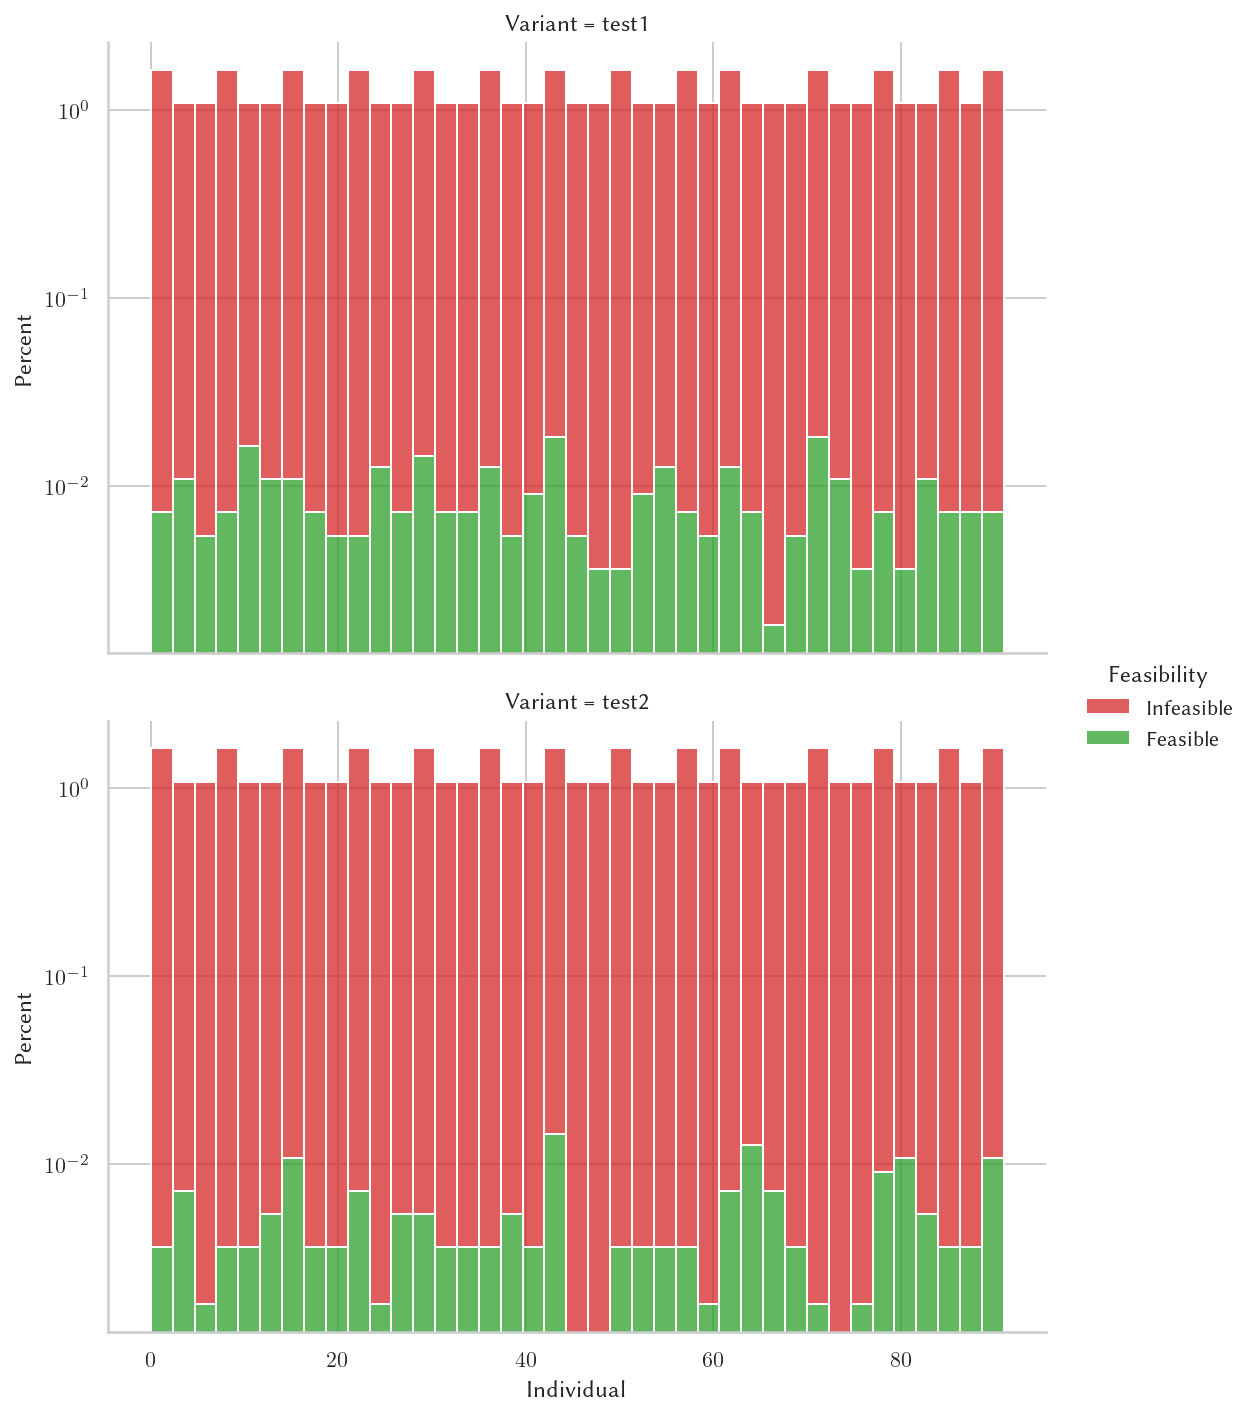
\includegraphics[width=.7\textwidth]{FeasibleInfeasible12}
    \caption{Resulting initial population distribution of 92 randomly initialized individuals (100 trials)}
    \label{fig:feasibleinfeasiblecomp}
\end{figure}

\subsubsection{Feasibility-Based Initialization}\label{sec_feas}
A third approach to generating the initial population is applying a feasibility-based initialization. In this method, a randomly generated individual is first tested for its adherence to all defined constraints. An individual is deemed infeasible if it does not meet all constraint criteria. Feasible individuals are added to the starting population, while infeasible individuals are discarded. This process is repeated until a population size $N$ is attained. An issue with this approach is the large amount of time needed to generate population size $N$. Depending on the population size $N$ and the number of objectives used, more computational time is often needed to obtain $N$ feasible individuals. Hence, algorithm variants using this approach are assigned a smaller population size.


\subsubsection{Hybrid Initialization}
The hybrid approach to initial population generation implemented in this thesis comprises feasibility-based and similarity-based initialization. In this approach, the similarity metric described in \ref{sec_sim} is first applied to generate a ranking of the regions. Regions having a rank below 0.7 are removed from further consideration. Next, possible region combinations are randomly generated, and only feasible individuals of size $N$ are allowed into the starting population.


\subsection{Constraint Handling Technique}
Handling of constraints and evaluation of the fitness of individuals in \gls{DEAP} are tightly coupled due to the interfaces provided in the framework. In this section, two approaches implemented for handling constraints are described. In both approaches, the constrained objective function is transformed into an unconstrained objective function by applying penalty functions.

\subsubsection{Distance-Based Penalties}
In this approach, the fitness value of infeasible individuals is replaced with a penalized fitness value $f^\mathrm{penalty}_i(x)$ using the penalty metric shown below:
\begin{align*}
    f^\mathrm{penalty}_i(\mathbf{x}) = \Delta_i - \sum_{j=1}^{N_{con}} d_{ij}(\mathbf{x})
\end{align*}
where $\Delta_i$ is the smallest possible score any individual of the population could obtain. In our case, $\Delta_i$ is set as $[0,0,0]$. $N_{con}$ represents the total constraints defined in our problem formulation (i.e., $N_{con} = 5$). $d_{ij}$ sums the distance of the individual to the feasible region for each constraint $j$. Depending on the constraint, each region that comprises an individual is penalized independently. Specifically, for the budget (\ref{eq:3_1b}) and duration (\ref{eq:3_1c}) constraints, $d_i^k$ for a specific region in individual $i$ is computed as follows:

\begin{align*}
    d_i^k =  \frac{c_k}{CV_i(x) * q_k} 
\end{align*}
$CV_i(x)$ is the sum over the normalized constraints and represents the degree of constraint violation of individual $i$ as described in Equation \ref{eq:4c}. $c_k$ is the actual budget or duration needed for the region $k$, while $q_k$ is the user-input budget or duration.

Regions that in a combination violate Constraint \ref{eq:3_1e} are assigned the value $d_i^k = \frac{c_k}{q_k}$, where $c_k$ is the number of user preferences the region does not fulfill, and $q_k$ is the total number of user preferences. For all other constraints (\ref{eq:3_1f} and \ref{eq:3_1f2}), the region combinations are penalized together with a constant value.

\subsubsection{Quadratic Penalty}
This approach transforms the objective function $z_i(x)$ into an unconstrained objective fitness function of the following form:
\begin{align*}
    f_i(x) = z_i(x) - \sum_{j=1}^{N_{con}}P_j(x)
\end{align*}
The penalty function $P_j$ is a quadratic function of the penalty coefficient for a given constraint. In the implementation, the penalty coefficient was chosen as the constraint violation degree $CV_i(x)$ over all constraints. Thus, the fitness value of an individual$i$ is computed as follows:
\begin{align*}
    f_{i}(x) := \begin{cases}
                            z_i(x), &\text{if}\quad CV_i(x) \leq 0 ;\\
                            [CV_i(x)]^2, &\text{otherwise};
                             \end{cases}
\end{align*}
Preliminary tests show better results using a quadratic increase of the violation degree as opposed to a linear increase.

\section{Discussion}
In this chapter, we presented and described in great detail \gls{nsga}-III as the baseline algorithm chosen for implementing the solution to our optimization problem. We described various heuristic solutions implemented in this thesis to modify the baseline algorithm. The objective function of the initial problem formulation was transformed in order to better handle the defined constraints. An implication of this transformation is that feasible members of the population will dominate infeasible members during non-dominated sorting. The tournament selection procedure described in Algorithm \ref{alg:tournament_selection} was relaxed such that individuals having higher fitness values are prioritized. Comparison between individual degrees of constraint violation is thus eliminated. However, the niche preservation operation is still used to select between individuals having the same Pareto front.




